\textbf{Kurzfassung.} Untersucht wird, welches Gitter die reine Dreikörperenergie

T\_ν(Λ) = Σ' (\textbar x\textbar{} · \textbar y\textbar{} · \textbar x − y\textbar)\textsuperscript{−ν} (Summe über alle Gitterdreiecke durch den Ursprung)

bei fester Dichte minimiert. Das ist eine \textbf{mathematische Modellenergie} und beschreibt kein Material. In 2D ist sie bis auf einen Faktor die modulare Graphfunktion C\textsubscript{s,s,s}(τ) mit s = ν/2. Die Hauptergebnisse sind zwei \textbf{Sätze für den Grenzfall ν → ∞}:

\begin{itemize}
\tightlist
\item
  In 2D laufen die Minimierer gegen ein Rechteckgitter mit Seitenverhältnis √((√17 − 1)/2) ≈ 1,2496. Der Beweis ist vollständig und von Hand.
\item
  In 3D laufen sie gegen BCC. Der Beweis ist computergestützt.
\end{itemize}

Außerdem ist für \textbf{endliches ν computergestützt bewiesen}, dass C₂,₂,₂, C₃,₃,₃ und C₄,₄,₄ ihr Minimum genau beim Quadratgitter τ = i haben (ν = 4, 6, 8). C₁,₁,₁ ist dagegen beim Hexagon minimal (klassisch).

Dazu kommen für endliches ν ein numerisches 2D-Phasendiagramm mit Fehlerbalken (hexagonal → Quadrat → Rechteck) und ein zertifizierter Einschluss des ersten Übergangs. Außerdem gibt es numerische Ergebnisse zu hcp, zu gemischten Energien aus Paar- und Dreikörperterm und zu ungleichen Exponenten.

\section{Einordnung: Was dieses Dokument behauptet und was nicht}

\begin{itemize}
\tightlist
\item
  \textbf{Mathematik-Geschichte, nicht Physik-Geschichte.} Echte Dreikörperkräfte (Axilrod--Teller--Muto) haben einen Winkelfaktor und treten immer zusammen mit Paarkräften auf. Aussagen über T\_ν gelten nur für diese Modellenergie.
\item
  \textbf{Geschenkt ist:} Hexagon und Quadrat sind Fixpunkte der Modulgruppe und deshalb für jede isometrieinvariante Energie kritische Punkte. BCC ist auf dem Bain-Pfad stationär; das ist bekannt (arXiv:2504.07338, Anhang H). Dass T\textsubscript{2s} = π\textsuperscript{3s} C\textsubscript{s,s,s} gilt, ist per Konstruktion bekannt (dieselbe Gittersumme).
\item
  \textbf{Inhalt haben:} die \textbf{globale} Minimalität, die Lage der Übergänge und die beiden Sätze im Limes.
\item
  \textbf{Die Summe selbst} ist die „three-body zeta function`` ζ⁽³⁾(ν,ν,ν) aus der Gruppe Buchheit/Schwerdtfeger (arXiv:2504.07338, 2504.11989). Dort wurde sie für einzelne Gitter und entlang des Bain-Pfads ausgewertet, aber nicht über alle Gitter minimiert.
\end{itemize}

\section{Ergebnisse auf einen Blick}

\begin{longtable}[]{@{}
  >{\raggedright\arraybackslash}p{(\columnwidth - 2\tabcolsep) * \real{0.5464}}
  >{\raggedright\arraybackslash}p{(\columnwidth - 2\tabcolsep) * \real{0.4236}}@{}}
\toprule\noalign{}
\begin{minipage}[b]{\linewidth}\raggedright
Aussage
\end{minipage} & \begin{minipage}[b]{\linewidth}\raggedright
Status
\end{minipage} \\
\midrule\noalign{}
\endhead
\bottomrule\noalign{}
\endlastfoot
2D: max. kleinstes Dreiecksprodukt P(Λ) ist P* = 2((1+√17)/8)\textsuperscript{3/4}, nur für das Rechteck mit Seitenverhältnis √((√17−1)/2) & \textbf{bewiesen} (Satz 1) \\
2D: Minimierer von T\_ν → dieses Rechteck für ν → ∞; ebenso das Minimum von C\textsubscript{s,s,s} für s → ∞ & \textbf{bewiesen} (Satz 2) \\
3D: max. P(Λ) = 3/2, nur für BCC; Minimierer von T\_ν → BCC für ν → ∞ & \textbf{computergestützt bewiesen} (Satz 3) \\
2D: C₂,₂,₂, C₃,₃,₃, C₄,₄,₄ haben ihr globales Minimum nur bei τ = i (Quadrat); ebenso T\_ν für ν = 5, 7; Hexagon ist einziger Minimierer bei ν = 3,5 & \textbf{computergestützt bewiesen} (Satz 4) \\
2D: Hexagon und Quadrat tauschen bei ν̂ ∈ (3,918364; 3,918366) die Reihenfolge & \textbf{zertifiziert} (explizite Fehlerschranken) \\
2D: global optimal ist hexagonal für 4/3 \textless{} ν \textless{} 3,91836, Quadrat bis ν₂ = 8,6063 ± 0,0005, danach Rechteck & numerisch, mit Fehlerbalken (Vermutung) \\
2D: beide Gitter lokal stabil für 3,80632 \textless{} ν \textless{} 4,27848 (Übergang erster Ordnung) & numerisch, Fehler ≤ 6·10⁻⁵ \\
3D: BCC bestes Gitter für alle getesteten ν von 2,2 bis 16 & numerisch (globale Suche bzw. Vergleich) \\
3D: FCC wird entlang des Bain-Pfads instabil bei ν\textsubscript{c} = 3,7521 ± 0,0001 & numerisch, mit Fehlerbalken \\
3D: hcp (optimales c/a) liegt stets knapp über FCC & numerisch \\
Paar + λ · Dreikörper: in 3D Sprung FCC → BCC bei λ\textsubscript{c}(ν), in 2D hexagonal → Quadrat & numerisch \\
\end{longtable}

\section{Satz 1 und 2: der Grenzfall ν → ∞ in 2D}

Für ein Gitter Λ sei P(Λ) das kleinste Produkt der drei gegenseitigen Abstände unter allen Tripeln verschiedener Gitterpunkte. Kollineare Tripel zählen mit. Sei a* = ((1+√17)/8)\textsuperscript{1/4} ≈ 0,894563, P* = 2a*³ ≈ 1,431734 und Λ* das Rechteckgitter mit Seiten a* und 1/a*.

\textbf{Satz 1.} Für jedes 2D-Gitter mit Kovolumen 1 gilt P(Λ) ≤ P*, mit Gleichheit genau für Λ* (bis auf Isometrie).

\textbf{Beweis.}

\begin{enumerate}
\def\labelenumi{\arabic{enumi}.}
\tightlist
\item
  Jedes Gitter hat nach Drehung und Spiegelung eine reduzierte Basis u = (a, 0), v = (p, 1/a) mit a = kürzeste Vektorlänge, 0 ≤ p ≤ a/2. Es gilt a⁴ ≤ 4/3 (Hermite-Konstante).
\item
  Das kollineare Tripel (0, u, 2u) hat Produkt 2a³.
\item
  Das Tripel (0, u, v) hat Produkt π mit π² = a²(p² + k)((a−p)² + k), wobei k = a\textsuperscript{−2}. Mit m = p(a − p) ∈ {[}0, a²/4{]} folgt (p²+k)((a−p)²+k) = (ka² + k²) + m(m − 2k). Wegen m ≤ a²/4 \textless{} 2k ist der letzte Summand ≤ 0, mit Gleichheit nur für p = 0. Also π ≤ √(a² + a\textsuperscript{−2}), mit Gleichheit nur beim Rechteck.
\item
  Somit P(Λ) ≤ G(a) := min(2a³, √(a² + a\textsuperscript{−2})). Der erste Term wächst in a, der zweite fällt auf (0, 1{]}. Sie schneiden sich genau bei 4a⁸ = a⁴ + 1, also a = a*. Für 1 ≤ a ≤ (4/3)\textsuperscript{1/4} ist a² + a\textsuperscript{−2} ≤ 7/(2√3), und das liegt unter P*². Daher ist G(a) ≤ P* mit Gleichheit nur für a = a*. Mit Schritt 3 folgt Gleichheit in Satz 1 nur für a = a* und p = 0, also für Λ*.
\item
  Umgekehrt ist P(Λ*) = P*:

  \begin{itemize}
  \tightlist
  \item
    Kollineare Tripel haben ein Produkt von mindestens 2s³ ≥ 2a*³, weil der Punktabstand s auf einer Gittergeraden mindestens a* ist.
  \item
    Ein nicht-kollineares Dreieck hat Fläche ≥ 1/2. Für die beiden kürzeren Seiten d₁, d₂ gilt daher d₁d₂ ≥ 1, also Produkt ≥ längste Seite d₃.
  \item
    Gittervektoren kürzer als D = √(a*² + a*\textsuperscript{−2}) sind nur ±u und ±v. Sie spannen nur zwei Richtungen auf, die drei Seiten eines Dreiecks aber drei paarweise unabhängige. Also ist d₃ ≥ D = P*. ∎
  \end{itemize}
\end{enumerate}

\textbf{Satz 2.} Für jedes ν \textgreater{} 4/3 hat T\_ν Minimierer. Jede Familie von Minimierern konvergiert für ν → ∞ gegen Λ*, und (min T\_ν)\textsuperscript{1/ν} → 1/P*. Für die modulare Graphfunktion bedeutet das: Die Minimalstellen von C\textsubscript{s,s,s} auf der Fundamentaldomäne konvergieren für s → ∞ gegen τ = i·√((√17−1)/2).

\textbf{Beweisidee.}

\begin{itemize}
\tightlist
\item
  T\_ν(Λ) ≥ P(Λ)\textsuperscript{−ν}, denn das kleinste Dreieck kommt in der Summe vor.
\item
  T\_ν(Λ*) ≤ C · P*\textsuperscript{−ν}.
\item
  Daraus folgt P(Λ\_ν) ≥ C\textsuperscript{−1/ν} P* → P*.
\item
  Mit Mahlers Kompaktheitssatz und Satz 1 konvergiert Λ\_ν gegen Λ*. ∎
\end{itemize}

Beide Sätze wurden numerisch gegengeprüft (\texttt{research/theorem/check\_maxmin\_2d.py}):

\begin{itemize}
\tightlist
\item
  20.000 Zufallsgitter verletzen die Schranke aus Schritt 4 nie.
\item
  Das numerische Maximum von P über die Fundamentaldomäne liegt bei τ ≈ 1,2475i.
\item
  Die berechneten Optima für endliches ν nähern sich monoton dem Grenzwert: 1,056 (ν=9), 1,100 (10), 1,141 (12), 1,170 (15), 1,194 (20), 1,215 (30).
\end{itemize}

\section{Satz 3: der Grenzfall ν → ∞ in 3D (computergestützt)}

\textbf{Satz 3.} Für jedes 3D-Gitter mit Kovolumen 1 gilt P(Λ) ≤ 3/2, mit Gleichheit genau für BCC. Folglich konvergieren die Minimierer von T\_ν (ν \textgreater{} 2) für ν → ∞ gegen BCC.

Zum Vergleich: P(FCC) = P(SC) = P(hcp) = √2 ≈ 1,414.

\textbf{Beweisaufbau.} Es sei Q(G) = P/√det G mit der Gram-Matrix G und G₁₁ = 1. Die übrigen fünf Einträge sind die Parameter.

\begin{enumerate}
\def\labelenumi{\arabic{enumi}.}
\tightlist
\item
  \textbf{Kompakter Suchbereich (von Hand bewiesen).}

  \begin{itemize}
  \tightlist
  \item
    Jedes Gitter hat eine Minkowski-reduzierte Gram-Matrix in einem expliziten Bereich 𝓡.
  \item
    Auf 𝓡 gilt det G ≥ g₂₂g₃₃/4. Das folgt aus dem Umkreisradius des spitzen Basisdreiecks und der Voronoi-Eigenschaft von b₃.
  \item
    Mit dem kollinearen Tripel folgt Q \textless{} 3/2, sobald g₂₂g₃₃ \textgreater{} 64/9. Übrig bleibt eine kompakte Box.
  \item
    BCC hat in 𝓡 genau einen Vertreter q₀ = (1, 1, 1/3, 1/3, −1/3).
  \end{itemize}
\item
  \textbf{Lokales Lemma (Intervallarithmetik).}

  \begin{itemize}
  \tightlist
  \item
    An q₀ sind 36 Dreiecke aktiv, mit 6 verschiedenen Gradienten. Deren konvexe Hülle enthält den Ursprung mit Abstand c = 0,13887.
  \item
    Jede Verformung senkt also mindestens eines dieser Dreiecke linear.
  \item
    Auf der Box q₀ ± 0,007 gilt streng ‖Hess f\textsubscript{t}‖ ≤ 14,92.
  \item
    Daraus folgt Q \textless{} 3/2 in der ganzen Box außer in q₀.
  \end{itemize}
\item
  \textbf{Branch-and-Bound über den Rest.}

  \begin{itemize}
  \tightlist
  \item
    Auf jeder Teilbox wird Q nach oben abgeschätzt, durch Maxima der (linearen) quadrierten Seitenlängen und ein Minimum der Determinante.
  \item
    Nach 9,93 Millionen Boxen ist \textbf{jede Box zertifiziert}: überall Q \textless{} 3/2.
  \end{itemize}
\end{enumerate}

\textbf{Status.} Das lokale Lemma ist streng, weil es mit Intervallarithmetik gerechnet ist. Der Branch-and-Bound rechnet in doppelter Genauigkeit mit Sicherheitsmargen (10⁻⁹ relativ, 10⁻¹² absolut). Diese übersteigen die Rundungsfehler der wenigen Rechenschritte pro Schranke um Größenordnungen. Ein vollständiger Neulauf in Intervallarithmetik ist möglich und steht noch aus. Kontrollen (\texttt{research/theorem3d/test\_prover.py}):

\begin{itemize}
\tightlist
\item
  In 1200 Stichproben lagen die Box-Schranken nie unter dem echten Wert.
\item
  Mit dem falschen Ziel 1,49 scheitert der Beweiser wie erwartet.
\end{itemize}

\section{Satz 4: endliches ν -- das Minimum von C₂,₂,₂, C₃,₃,₃, C₄,₄,₄}

\textbf{Satz 4.} Für s = 2, 3, 4 nimmt die modulare Graphfunktion C\textsubscript{s,s,s}(τ) ihr Minimum auf der Fundamentaldomäne nur bei τ = i an. Gleichwertig: Für ν = 4, 6, 8 ist das Quadratgitter der einzige Minimierer von T\_ν.

Zusammen mit dem klassischen Fall s = 1 (Minimum beim Hexagon) und Satz 2 ergibt sich:

\begin{itemize}
\tightlist
\item
  s = 1: Minimum beim Hexagon;
\item
  s = 2, 3, 4: Minimum beim Quadrat;
\item
  s → ∞: Minimum gegen das Rechteck mit Seitenverhältnis 1,2496.
\end{itemize}

\textbf{Die Idee, die den Beweis handhabbar macht: eine universelle Majorante.}

\begin{itemize}
\tightlist
\item
  Schreibt man die quadrierte Seitenlänge eines Gittervektors in τ-Koordinaten, dann ist ihre relative Änderung koeffizientenweise durch eine einzige Reihe ε̂(A,B) = (A + B + A² + B²)/(1 − B) beschränkt, für \textbf{jeden} Gittervektor.
\item
  Daher sind alle Taylor-Koeffizienten von T durch T(τ₀) mal den Koeffizienten von (1 − ε̂)\textsuperscript{−3s} beschränkt.
\item
  Das liefert explizite Restglieder und explizite Schranken für die abgeschnittenen Summanden.
\end{itemize}

\textbf{Beweisaufbau.}

\begin{enumerate}
\def\labelenumi{\arabic{enumi}.}
\tightlist
\item
  \textbf{Großes Im τ:} Für Im τ \textgreater{} Y₀ ist T schon wegen der kollinearen Tripel größer als T(i).
\item
  \textbf{Lokales Lemma bei i:} Die Symmetrien x ↦ −x und τ ↦ 1/τ̄ lassen i fest und erzwingen, dass die Taylor-Koeffizienten c₁₀, c₀₁, c₁₁, c₃₀, c₁₂ verschwinden. Mit streng eingeschlossenen c₂₀, c₀₂, c₂₁, c₀₃ und der Majorante folgt T \textgreater{} T(i) in einer Box um i.
\item
  \textbf{Branch-and-Bound über den Rest:} Taylor-Entwicklung zweiter Ordnung am Boxmittelpunkt mit streng eingeschlossenen Koeffizienten, minus Majoranten-Restglied, liegt über T(i). Die Koeffizienten stammen aus direkten Faltungen ohne FFT, mit expliziter Schranke für den abgeschnittenen Rest und Rundungsmarge.
\end{enumerate}

\begin{longtable}[]{@{}
  >{\raggedright\arraybackslash}p{(\columnwidth - 10\tabcolsep) * \real{0.1667}}
  >{\raggedright\arraybackslash}p{(\columnwidth - 10\tabcolsep) * \real{0.1667}}
  >{\raggedright\arraybackslash}p{(\columnwidth - 10\tabcolsep) * \real{0.1667}}
  >{\raggedright\arraybackslash}p{(\columnwidth - 10\tabcolsep) * \real{0.1667}}
  >{\raggedright\arraybackslash}p{(\columnwidth - 10\tabcolsep) * \real{0.1667}}
  >{\raggedright\arraybackslash}p{(\columnwidth - 10\tabcolsep) * \real{0.1667}}@{}}
\toprule\noalign{}
\begin{minipage}[b]{\linewidth}\raggedright
ν
\end{minipage} & \begin{minipage}[b]{\linewidth}\raggedright
T(i) eingeschlossen in
\end{minipage} & \begin{minipage}[b]{\linewidth}\raggedright
c₂₀ ≥
\end{minipage} & \begin{minipage}[b]{\linewidth}\raggedright
c₀₂ ≥
\end{minipage} & \begin{minipage}[b]{\linewidth}\raggedright
Radius lokales Lemma
\end{minipage} & \begin{minipage}[b]{\linewidth}\raggedright
Boxen
\end{minipage} \\
\midrule\noalign{}
\endhead
\bottomrule\noalign{}
\endlastfoot
4 & {[}7,5826697721; 7,5826700248{]} & 0,43688 & 9,75784 & 0,0031 & 531 \\
5 & {[}4,8380268461; 4,8380268473{]} & 2,58218 & 6,30394 & 0,0070 & 303 \\
6 & {[}3,2499743121; 3,2499743128{]} & 4,27194 & 3,57092 & 0,0076 & 307 \\
7 & {[}2,2334461746; 2,2334461750{]} & 5,34452 & 1,66169 & 0,0050 & 323 \\
8 & {[}1,5524012124; 1,5524012128{]} & 5,83081 & 0,46080 & 0,0026 & 385 \\
\end{longtable}

Zusätzlich sind so auch ν = 5 und ν = 7 bewiesen (keine modularen Graphfunktionen, da s nicht ganzzahlig). Das Quadrat ist also an fünf Stützstellen ν = 4, 5, 6, 7, 8 nachweislich optimal. Das kleine c₀₂ bei ν = 8 zeigt die Nähe des Übergangs zum Rechteck bei ν₂ ≈ 8,606.

\textbf{Auch das Hexagon ist so beweisbar:} Bei ν = 3,5 ist das Hexagonalgitter der einzige Minimierer (T(ρ) ∈ {[}9,7723429; 9,7724089{]}, Radius des lokalen Lemmas 0,0072, 363 Boxen). Damit ist die Phasenfolge an Stützstellen auf beiden Seiten von ν* bewiesen: Hexagon bei ν = 2 (klassisch) und 3,5, Quadrat bei ν = 4 bis 8.

\textbf{Grenze der Methode:} Der gleiche Beweis für das Hexagon bei ν = 3 ist gescheitert. Nahe ν = d fällt der abgeschnittene Rest nur wie R⁻⁴ ab. Mit R = 40 ist die Fehlerschranke (≈ 10⁻³) größer als der Energieabstand direkt neben dem Hexagon. Dafür bräuchte es deutlich größere Summen oder eine schärfere Schranke für den Rest. \textbf{Status:} wie bei Satz 3. Die Rechnung läuft in doppelter Genauigkeit mit expliziten Margen, nicht vollständig in Intervallarithmetik. Skripte: \texttt{research/theorem\_mgf/}.

\section{Endliches ν in 2D (Numerik mit Fehlerangaben)}

Die Rechnungen verwenden eine eigene Referenzsumme ohne GZL-Code. Die Übereinstimmung mit GZL liegt bei 55 Testfällen unter 2·10⁻¹⁰, und die Werte bei ν = 3 stimmen mit arXiv:2504.07338 überein.

\begin{itemize}
\tightlist
\item
  \textbf{4/3 \textless{} ν \textless{} 3,91836: hexagonal.}

  \begin{itemize}
  \tightlist
  \item
    Bei ν = 2 ist das exakt, weil T₂ = π³(E₃ + ζ(3)) und die Epstein-Zeta ihr Minimum beim Hexagon hat.
  \item
    Für 1,4 ≤ ν ≤ 1,9 ist das Hexagon unter den Kandidaten am tiefsten, stabil auf 10⁻⁸. Dafür war ein Hochrechnungsansatz mit zwei Exponentenfamilien nötig.
  \end{itemize}
\item
  \textbf{Übergang bei ν*:} Der Wechsel von hexagonal zu Quadrat ist zertifiziert in (3,918364; 3,918366).

  \begin{itemize}
  \tightlist
  \item
    Dafür wurde die abgeschnittene Summe direkt gefaltet, ohne FFT.
  \item
    Der Rest ist explizit abgeschätzt, und für Rundung gibt es eine Marge (\texttt{research/theorem/certify\_nustar.py}).
  \end{itemize}
\item
  \textbf{Erste Ordnung:} Das Quadrat ist lokal stabil ab 3,80632, das Hexagon bis 4,27848. Bei ν* liegt auf dem Bogen \textbar τ\textbar{} = 1 eine Barriere von 0,14 \%.
\item
  \textbf{ν₂ = 8,6063 ± 0,0005:} Dort wird das Quadrat in Streckrichtung instabil. Danach ist das Optimum ein Rechteck, dessen Seitenverhältnis gegen 1,2496 wächst (Satz 2).
\end{itemize}

\begin{figure}
\centering

\includegraphics{../verification/figures/fig_2d_energy_difference.pdf}
\caption{Energiedifferenz zum Hexagonalgitter: Quadrat (Linie) und bestes Rechteck (Punkte).}
\end{figure}

\begin{figure}
\centering

\includegraphics{../verification/figures/fig_2d_stability.pdf}
\caption{Kleinster Hesse-Eigenwert von Hexagon und Quadrat; grau: Koexistenzbereich.}
\end{figure}

\begin{figure}
\centering

\includegraphics[width=1\textwidth,height=\textheight]{../verification/figures/fig_2d_landscape.pdf}
\caption{Energielandschaft über der Fundamentaldomäne bei vier Exponenten.}
\end{figure}

\textbf{Vermutung.} In 2D ist der Minimierer hexagonal für 4/3 \textless{} ν \textless{} ν*, quadratisch für ν* \textless{} ν ≤ ν₂ und rechteckig mit wachsendem Seitenverhältnis für ν \textgreater{} ν₂.

\section{Endliches ν in 3D (Numerik)}

\begin{itemize}
\tightlist
\item
  \textbf{Globale Suche über alle Bravais-Gitter:} 67 Starts pro ν (FCC, BCC, SC und 64 zufällige), Nelder-Mead mit genauer Nachberechnung (\texttt{research/extended/e1\_3d\_search.py}). Für ν = 3,2; 3,5; 4; 4,5; 6 ist das beste gefundene Gitter jedes Mal BCC, auf 10⁻⁹ relativ. 87--100 \% aller Starts laufen nach BCC. Weitere ν-Werte laufen noch; sie werden in \texttt{research/extended/results/} ergänzt.
\item
  \textbf{Kleine ν (2,2 bis 2,8):} BCC \textless{} FCC \textless{} SC, stabil über zwei Abschneide-Sätze.
\item
  \textbf{FCC-Instabilität:} Die Krümmung entlang des Bain-Pfads wechselt bei ν\textsubscript{c} = 3,7521 ± 0,0001 das Vorzeichen. Der Fehlerbalken ist die Streuung über drei Schrittweiten und zwei Abschneide-Sätze. Die instabile Richtung zeigt zu BCC.
\item
  \textbf{hcp:} Über c/a ∈ {[}1,45; 1,85{]} optimiert liegt hcp bei allen getesteten ν knapp über FCC, zum Beispiel 17,9724 gegenüber 17,9624 bei ν = 4,5, mit BCC bei 17,7406.
\end{itemize}

\section{Gemischte Energien: Paar- plus Dreikörperterm}

E\_λ = Z\_ν + λ · T\_ν mit der Paarenergie Z\_ν = Σ'\textbar x\textbar{}\textsuperscript{−ν} (gleicher Abfall pro Bindung) bei fester Dichte. Z\_ν wurde exakt mit epsteinlib berechnet.

\begin{longtable}[]{@{}lll@{}}
\toprule\noalign{}
ν & 3D: λ\textsubscript{c} (FCC → BCC) & 2D: λ\textsubscript{c} (hexagonal → Quadrat) \\
\midrule\noalign{}
\endhead
\bottomrule\noalign{}
\endlastfoot
3,0 & -- & kein Übergang (Hexagon für alle λ) \\
3,5 & 0,049 & -- \\
4,5 & 0,065 & 1,861 \\
6,0 & 0,103 & 1,044 \\
9,0 & 0,289 & 1,507 (Rechteck ab λ ≈ 200) \\
\end{longtable}

\begin{itemize}
\tightlist
\item
  In 3D springt das Optimum unter den Kandidaten direkt von FCC zu BCC; \textbf{hcp ist nie optimal}.
\item
  In 2D gab es auf dem Gitter der Fundamentaldomäne kein Zwischengitter.
\item
  Die Kandidatenmenge in 3D ist FCC, BCC, hcp(c/a) und die Bain-Familie. Eine globale Suche für gemischte Energien steht noch aus.
\end{itemize}

\section{\texorpdfstring{Ungleiche Exponenten C\textsubscript{a,a,b}}{Ungleiche Exponenten Ca,a,b}}

Gesucht wurde der globale Minimierer von Σ' \textbar x\textbar{}\textsuperscript{\{−ν\}\textbar y\textbar{}}\{−ν\}\textbar x−y\textbar{}\textsuperscript{−μ} über der ganzen Fundamentaldomäne, auf einem Gitter ν, μ ∈ {[}2,5; 12{]} mit Schrittweite 0,5. Das ist bis auf Normierung C\_\{ν/2, ν/2, μ/2\}. Aus der Kurve im Fall gleicher Exponenten wird damit eine Phasenfläche:

\begin{itemize}
\tightlist
\item
  \textbf{Hexagonal} ist optimal, wenn alle Exponenten klein sind (ν ≲ 3,5) oder wenn einer deutlich kleiner ist als die anderen.
\item
  \textbf{Quadrat} ist in einem breiten Band um die Diagonale optimal. Für 4 ≤ ν ≤ 5,5 kehrt bei großem μ das \textbf{Hexagon zurück}; das Quadratfenster schließt sich also nach oben.
\item
  \textbf{Rechteck} tritt nur für ν ≳ 9 in einem Fenster 8,5 ≲ μ ≲ 11 auf. Diese Phase gehört zum Übergang bei ν₂ auf der Diagonale.
\item
  Andere Gittertypen (rhombisch, schief) wurden nirgends gefunden.
\end{itemize}

Die Auflösung ist 0,5 in beiden Richtungen; die Grenzen sind entsprechend grob.

\begin{figure}
\centering
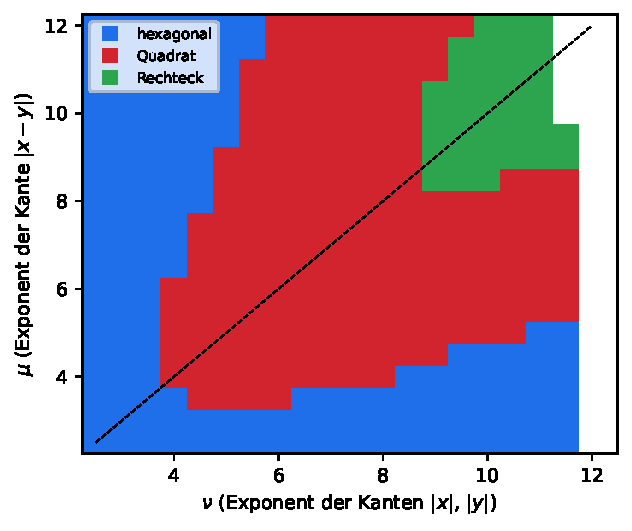
\includegraphics{../extended/figures/fig_e3_phase_map.pdf}
\caption{Optimales Gitter für die Exponenten (ν, ν, μ). Gestrichelt: gleiche Exponenten.}
\end{figure}

\begin{figure}
\centering
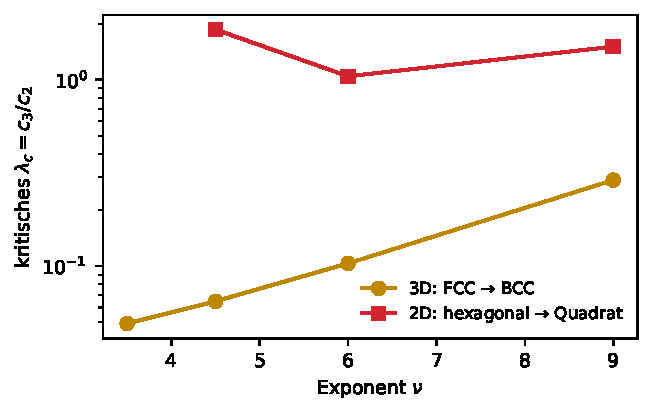
\includegraphics{../extended/figures/fig_e4_lambda_c.pdf}
\caption{Kritisches Verhältnis λ\textsubscript{c} = c₃/c₂ für Paar- plus Dreikörperenergie.}
\end{figure}

\section{Neuheit}

Drei Literaturprüfungen liefen über KI-Agenten: nach Stichworten, als Volltextsuche und Autor für Autor (Bétermin, Petrache, Faulhuber, Stefanelli/Friedrich/Kreutz, Luo--Wei, Cohn, Bilyk, Buchheit/Schwerdtfeger). Keine fand die Sätze 1--3 oder das Phasendiagramm. Am nächsten liegen:

\begin{itemize}
\tightlist
\item
  \textbf{arXiv:2504.07338:} dieselbe Summe, aber nur bei ν = 3 und nur auf dem Bain-Pfad.
\item
  \textbf{arXiv:2107.14020:} dieselbe Beweistechnik für große Exponenten, aber für Paarenergien.
\item
  \textbf{arXiv:2303.12283 (Bilyk u. a.):} Dreipunkt-Max-Min-Probleme auf der Sphäre, nicht auf Gittern.
\end{itemize}

Die Einschätzung der Agenten ist 85--90 \% für Satz 1/2 und etwa 65 \% für die 3D-Aussagen. Eine Garantie ist das nicht; Google Scholar war nicht erreichbar. Das \textbf{Risiko, dass jemand zuvorkommt, ist hoch}, weil die Gruppe Buchheit/Schwerdtfeger an Mehrkörper-Stabilität arbeitet.

\section{Grenzen und nächste Schritte}

\begin{itemize}
\tightlist
\item
  Für endliches ν sind jetzt die Fälle ν = 4, 6, 8 bewiesen (Satz 4) und ν* ist zertifiziert eingeschlossen. Offen bleibt das vollständige Phasendiagramm, etwa dass das Hexagon für \textbf{alle} ν \textless{} ν* optimal ist. Mit demselben Verfahren lassen sich weitere einzelne ν-Werte beweisen, ein Kontinuum aber nur mit zusätzlicher Arbeit.
\item
  Der Branch-and-Bound in 3D sollte noch vollständig in Intervallarithmetik laufen.
\item
  Die physikalisch relevante Frage mit Winkelfaktor (ATM) ist nicht behandelt.
\end{itemize}

\section{Reproduzierbarkeit}

Alle Pfade sind relativ zum Repository:

\begin{itemize}
\tightlist
\item
  \texttt{research/verification/}: Referenzsumme und Nachprüfung
\item
  \texttt{research/theorem/}: 2D-Satz und zertifiziertes ν*
\item
  \texttt{research/theorem3d/}: lokales Lemma, Branch-and-Bound und Tests (Satz 3)
\item
  \texttt{research/theorem\_mgf/}: Majorante, Taylor-Jets und Beweis für C₂,₂,₂, C₃,₃,₃, C₄,₄,₄ (Satz 4)
\item
  \texttt{research/extended/}: 3D-Suche, Fehlerbalken, hcp, gemischte Energien, ungleiche Exponenten, kleine ν
\item
  \texttt{research/note/}: englische Note mit allen Beweisen
\end{itemize}
